\documentclass[11pt, letterpaper]{article}
\usepackage[margin=1in]{geometry}
\usepackage{graphicx}
\usepackage{booktabs}
\usepackage{array}
\usepackage{hyperref}
\usepackage{enumitem}
\usepackage{titlesec}
\usepackage{xcolor}
\usepackage{fancyhdr}
\usepackage{tikz}
\usetikzlibrary{shapes.geometric, arrows.meta, positioning, fit, backgrounds}

\definecolor{green}{RGB}{46, 125, 50}
\definecolor{blue}{RGB}{21, 101, 192}
\definecolor{gray}{RGB}{97, 97, 97}

\hypersetup{colorlinks=true, linkcolor=blue, urlcolor=blue}

\pagestyle{fancy}
\fancyhf{}
\rfoot{Page \thepage}

\titleformat{\section}{\large\bfseries\color{green}}{}{0em}{}[\color{green}\titlerule]
\titleformat{\subsection}{\normalsize\bfseries}{}{0em}{}

\setlist[itemize]{noitemsep, topsep=2pt}

\begin{document}

% ── Title ──────────────────────────────────────────────────────────────────
\begin{center}
  {\LARGE\bfseries Multimodal Crop Health Monitoring}\\[6pt]
  {\large EGN6217 - Applied DEEP Learning}\\[10pt]
  {\normalsize Khang Phan - Spring 2026}\\[4pt]
  {\small \href{https://github.com/itsmekhang/crop-health-monitoring}{github.com/itsmekhang/crop-health-monitoring}}
\end{center}

\vspace{0.5em}
\hrule
\vspace{1em}

% ── Section 1 ──────────────────────────────────────────────────────────────
\section{Problem Context and Project Summary}

The agriculture industry has evolved rapidly in recent history and is now facing increasing pressure to efficiently use water, pesticides, and fertilizers, yet most farmers still rely on manual observation or delayed testing—leading to late disease detection, wasted resources, and reduced yields. This project builds a budget-friendly, modular AI system that detects crop diseases from leaf images using ResNet18 and assesses environmental risk from live weather values using gradient-boosted trees. The two models operate independently but are surfaced together through a Streamlit interface, giving farmers or researchers an interactive tool that combines visual and environmental insights in one interface. The system is designed to be scalable and extensible for future multimodal enhancements.

% ── Section 2 ──────────────────────────────────────────────────────────────
\section{Dataset}

\subsection{PlantVillage (Image Classification)}
\begin{itemize}
  \item \textbf{Source:} \href{https://www.kaggle.com/datasets/emmarex/plantdisease}{Kaggle — emmarex/plantdisease}
  \item \textbf{Type:} Labeled RGB leaf images, 224$\times$224 px after resizing
  \item \textbf{Size:} $\approx$54,000 images within 38 disease/healthy classes
  \item \textbf{Access:} Kaggle API — \texttt{kaggle datasets download -d emmarex/plantdisease}
  \item \textbf{Preprocessing:} Resize to 224$\times$224; normalize with ImageNet; augment with random flips, rotations ($\pm15°$), and color jitter
  \item \textbf{Challenges:} Class imbalance; controlled lab lighting may not generalize well
  \item \textbf{Ethics:} Publicly available
\end{itemize}

\subsection{USDA NASS QuickStats (Yield Baselines)}
\begin{itemize}
  \item \textbf{Source:} \href{https://quickstats.nass.usda.gov}{USDA National Agricultural Statistics Service — QuickStats API}
  \item \textbf{Type:} API returning crop yield prices, and environmental values by state and year
  \item \textbf{Crops:} Tomatoes, Potatoes, Bell Peppers — matching the disease model's crop coverage
  \item \textbf{Access:} Free API key from \href{https://quickstats.nass.usda.gov/api}{quickstats.nass.usda.gov/api}
  \item \textbf{Usage:} National average yield as the healthy-crop baseline for revenue loss estimation
  \item \textbf{Challenges:} US-specific data
  \item \textbf{Ethics:} Publicly funded government data; open access; no personal or sensitive information
\end{itemize}

% ── Section 3 ──────────────────────────────────────────────────────────────
\section{Planned Architecture}

\subsection{Data Flow Diagram}

\begin{center}
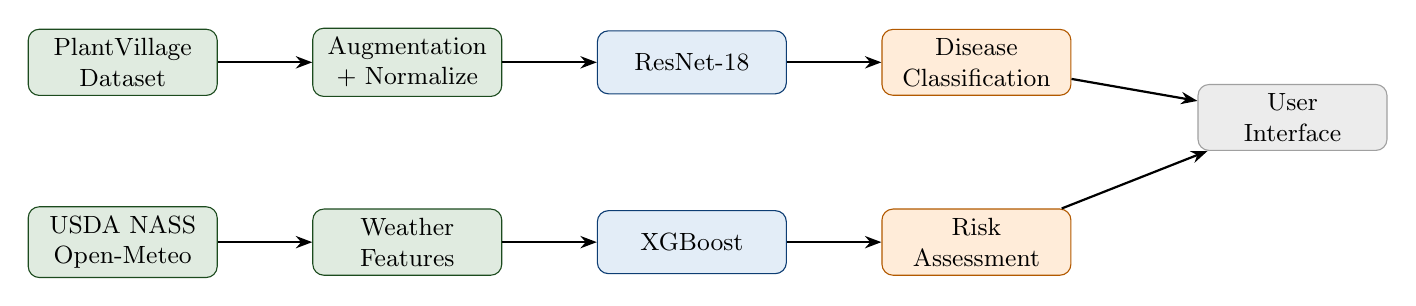
\begin{tikzpicture}[
  node distance=0.8cm and 1.2cm,
  box/.style={draw, rounded corners=4pt, minimum width=2.4cm, minimum height=0.8cm,
               align=center, font=\small},
  greenbox/.style={box, fill=green!15, draw=green!60!black},
  bluebox/.style={box,  fill=blue!12,  draw=blue!60!black},
  orangebox/.style={box, fill=orange!15, draw=orange!70!black},
  graybox/.style={box,  fill=gray!12,  draw=gray!60},
  arr/.style={-{Stealth[scale=0.9]}, thick},
]

% Image pipeline (top row)
\node[greenbox] (pv)    {PlantVillage\\Dataset};
\node[greenbox, right=of pv] (aug)   {Augmentation\\+ Normalize};
\node[bluebox,  right=of aug] (resnet) {ResNet-18};
\node[orangebox,right=of resnet] (dcls)  {Disease\\Classification};

% Risk pipeline (bottom row)
\node[greenbox, below=1.4cm of pv]   (csv)    {USDA NASS\\ Open-Meteo};
\node[greenbox, right=of csv] (feat)   {Weather\\Features};
\node[bluebox,  right=of feat] (xgb)    {XGBoost};
\node[orangebox,right=of xgb] (yreg)   {Risk\\Assessment};

% Dashboard
\node[graybox, right=1.6cm of dcls, yshift=-0.7cm] (ui) {User\\Interface};

% Arrows — image
\draw[arr] (pv)     -- (aug);
\draw[arr] (aug)    -- (resnet);
\draw[arr] (resnet) -- (dcls);
\draw[arr] (dcls)   -- (ui);

% Arrows — yield
\draw[arr] (csv)  -- (feat);
\draw[arr] (feat) -- (xgb);
\draw[arr] (xgb)  -- (yreg);
\draw[arr] (yreg) -- (ui);

\end{tikzpicture}
\end{center}

\vspace{0.5em}

\subsection{Image Model — Disease Classifier}
\begin{itemize}
  \item \textbf{Architecture:} ResNet-18 with ImageNet pretrained weights
  \item \textbf{Strategy:} Transfer learning
  \item \textbf{Fine-tuning:} After initial training, resume the last two ResNet blocks for domain adaptation
  \item \textbf{Loss:} CrossEntropyLoss
  \item\textbf{Optimizer:} Adam 
  \item \textbf{Target metric:} Validation accuracy $\geq$85\%
\end{itemize}

\subsection{Tabular Model — Environmental Risk Scorer}
\begin{itemize}
  \item \textbf{Main model:} XGBoost Regressor (n\_estimators=300, max\_depth=5)
  \item \textbf{Features:} temperature, humidity, days since rain, ResNet confidence, disease class
  \item \textbf{Target:} Risk score in  the range of $[0, 1]$ — derived from augmented disease-weather relationships
  \item \textbf{Weather source:} Open-Meteo API, fetched live by location at runtime
  \item \textbf{Yield baseline:} USDA NASS QuickStats API — national average yield per crop in lbs/acre
  \item \textbf{Achieved metric:} Validation R² = 0.998, Validation MAE = 0.008 on held-out split
\end{itemize}

\subsection{Interface}
The Streamlit user interface (\texttt{ui/app.py}) takes leaf image files, a location, and economic inputs (field size, crop price). Weather is fetched automatically from Open-Meteo using the location. The disease classifier analyzes the uploaded images; XGBoost scores risk from the disease result and live environmental conditions. Outputs return disease class, confidence, risk level, treatment plan, and estimated revenue loss. 

% ── Section 4 ──────────────────────────────────────────────────────────────
\section{User Interface Plan}

\subsection{Inputs and Outputs}

\begin{center}
\begin{tabular}{@{}lll@{}}
\toprule
\textbf{Section} & \textbf{User Input} & \textbf{Output Displayed} \\
\midrule
Leaf Images     & Upload one or more leaf photos & Disease class, confidence, top-5 predictions \\
Weather         & City or region name & Live temp, humidity, days since rain \\
Economic Impact & Field size, crop price & Yield loss, revenue loss  \\
\midrule
\multicolumn{2}{l}{\textit{Combined output per image}} & Risk score, risk level, treatment plan \\
\bottomrule
\end{tabular}
\end{center}

\subsection{Application Screenshots}

\begin{figure}[h]
  \centering
  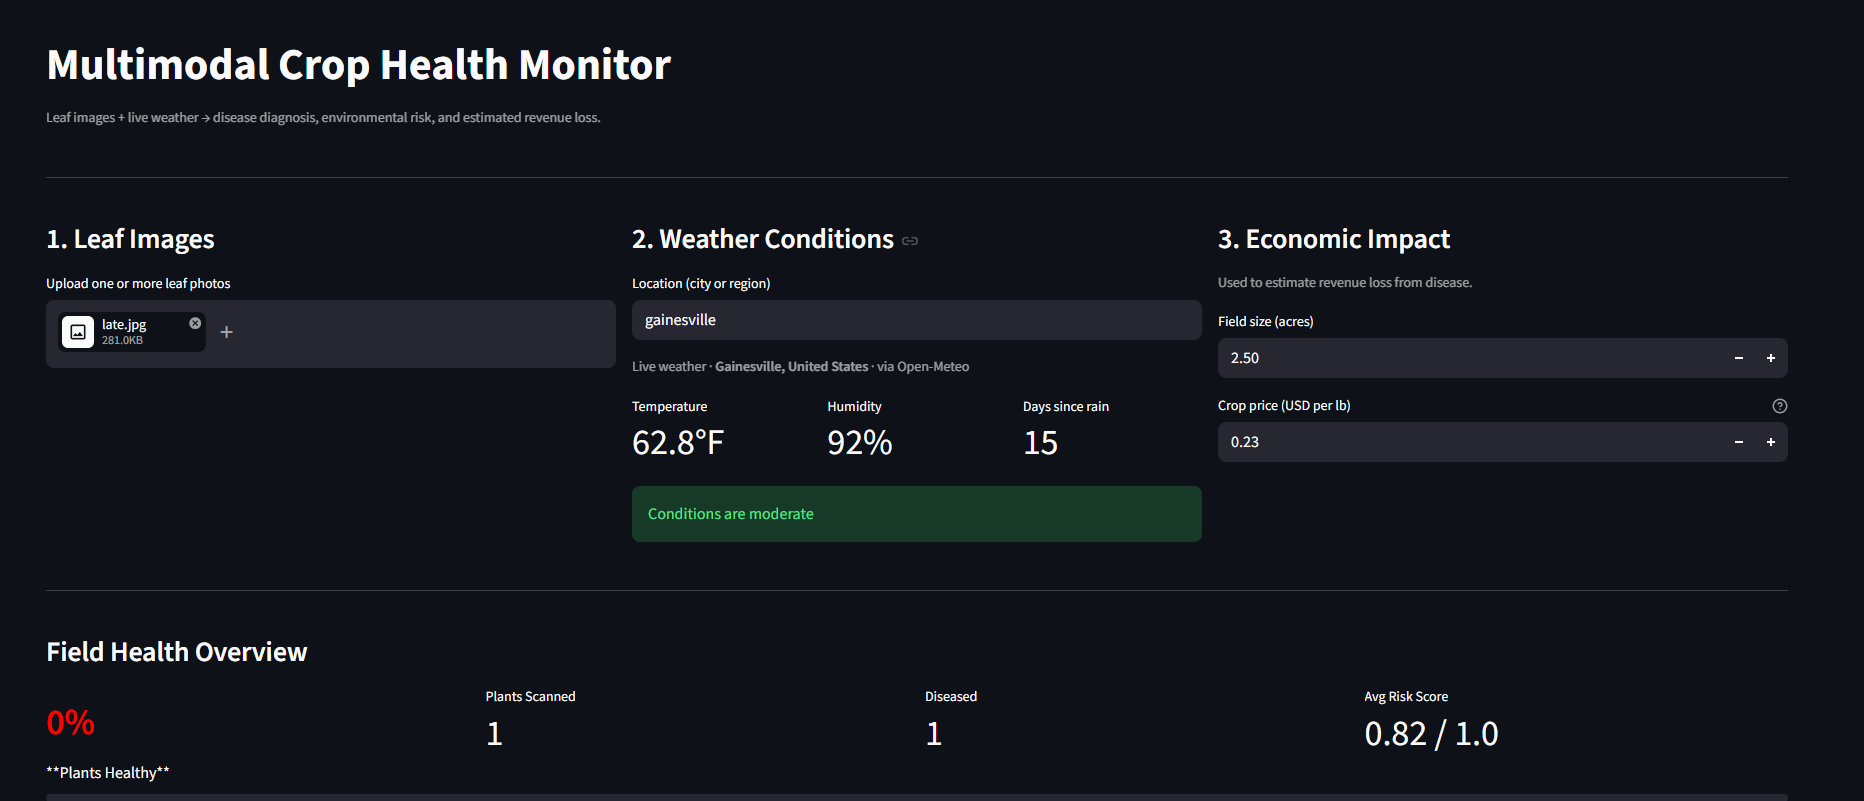
\includegraphics[width=\textwidth]{screenshot_input.png}
  \caption{Dashboard input panel — leaf image upload, live weather via Open-Meteo, and economic impact inputs.}

  \centering
  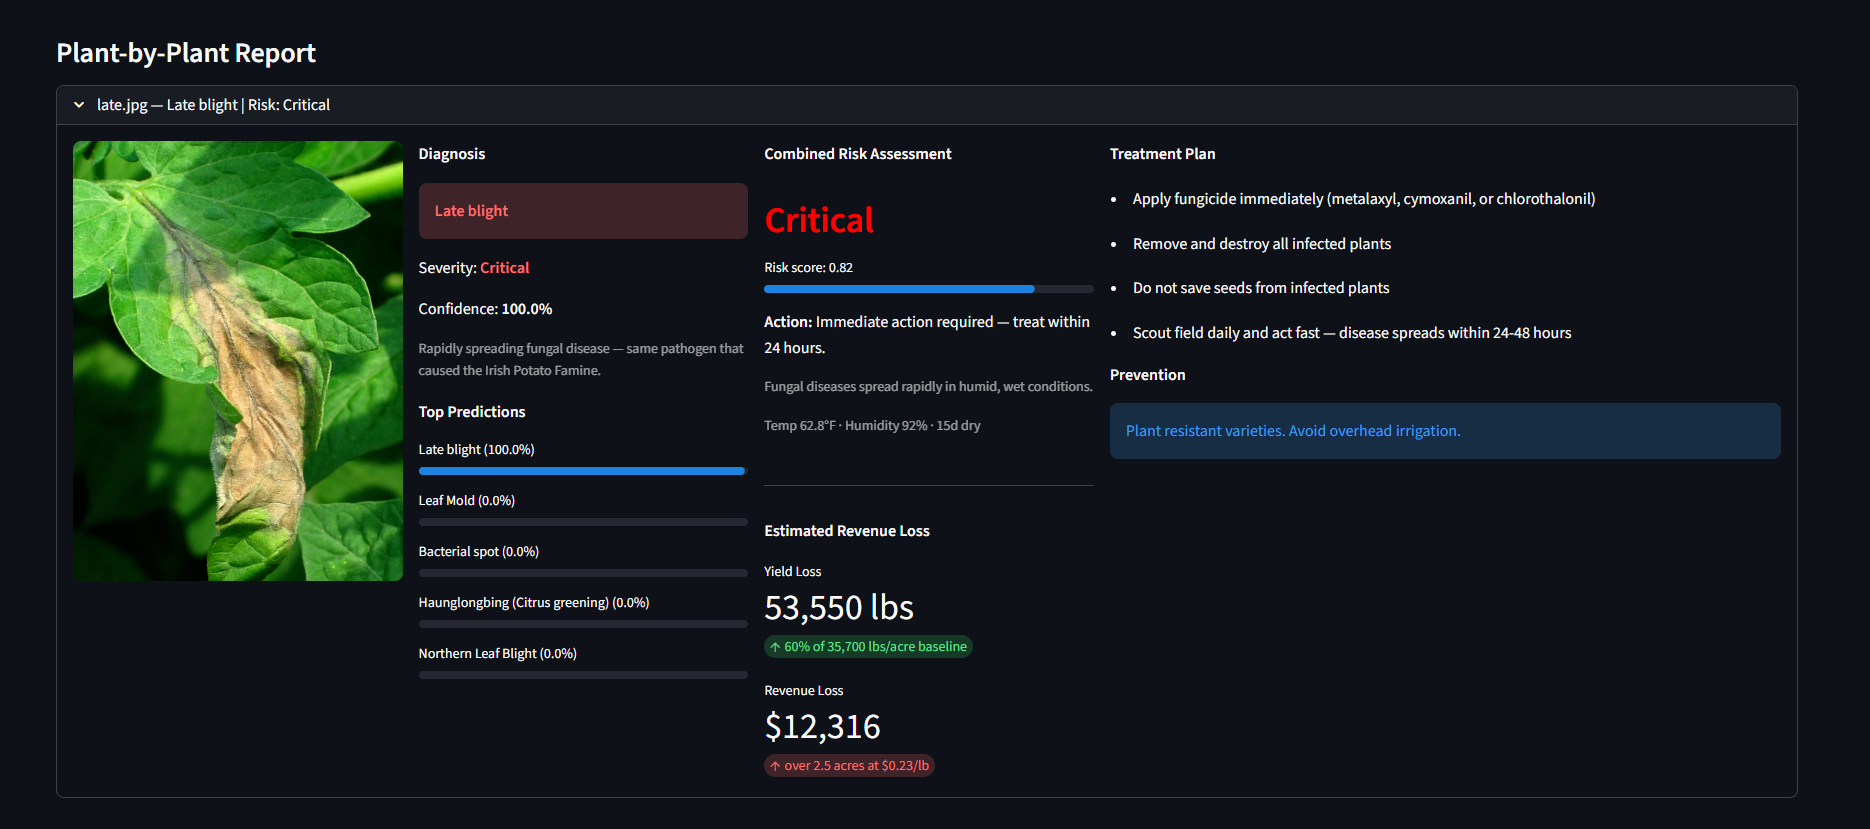
\includegraphics[width=\textwidth]{screenshot_output.png}
  \caption{Plant-by-Plant Report — disease diagnosis, XGBoost risk assessment, treatment plan, and estimated revenue loss.}
\end{figure}

% ── Section 5 ──────────────────────────────────────────────────────────────
\section{Innovation and Anticipated Challenges}

\subsection{Innovation}
This project is novel in its \textit{practical multimodal design}: rather than forcing a single fused model which is difficult to train and debug, it trains two separate models and combine them together through one interface. This modular approach lowers the complexity for farmers to use AI tools without requiring technical knowledge. The combination of transfer learning on PlantVillage and gradient-boosted trees on environmental data includes both early disease detection and seasonal yield planning.

% ── Section 6 ──────────────────────────────────────────────────────────────
\section{Implementation Timeline}

\begin{center}
\begin{tabular}{@{}>{\bfseries}p{2.8cm}p{4.5cm}p{5.5cm}@{}}
\toprule
Week & Focus & Expected Outcome \\
\midrule
Apr 5 – Apr 12 &
  Data collection, EDA, baseline models &
  Working data loaders; EDA plots in \texttt{setup.ipynb}; random forest baseline ($R^2 > 0.6$) \\
\addlinespace
Apr 12 – Apr 19 &
  ResNet-18 training; XGBoost tuning; metric tracking &
  Disease classifier $\geq$80\% val accuracy; XGBoost $R^2 \geq 0.80$; \texttt{results/} populated \\
\addlinespace
Apr 19 – Apr 26 &
  Streamlit UI build; model integration; demo run &
  Fully interactive dashboard; end-to-end inference working on both functionalities \\
\addlinespace
Apr 26 – Apr 29 &
  Final report, README polish, repo cleanup &
  Completed report; tidy repository; presentation-ready prototype \\
\bottomrule
\end{tabular}
\end{center}

% ── Section 7 ──────────────────────────────────────────────────────────────
\section{Responsible AI Reflection}

\textbf{Fairness:} The PlantVillage dataset was collected in consistent laboratory settings, which might not generalize well under a variety field conditions across different geographies, soil types, or lighting environments. A model trained only on this data could perform underwhelmingly for farmers in regions underrepresented in the dataset. Future work should evaluate performance separately by each crop class or conditions, and collect field images from real-world settings.

\textbf{Transparency:} The Streamlit interface shows top-5 class probabilities rather than a single hard prediction, giving users a sense of the model's desicion making. For the yield model, feature importance plots (saved to \texttt{results/}) make the model's reasoning inspectable.

\textbf{Environmental impact:} ResNet-18 is a relatively lightweight architecture. Training on a single GPU for 10 epochs on 54,000 images takes approximately 10-20 min. The XGBoost model is CPU-bound and trains in under a minute.

\textbf{Misuse risk:} Overconfident disease predictions could cause a farmer to implement the wrong mitigation technique or address the situation inappropriately. The UI is designed to communicate uncertainty to discourage overreliance on the model not being robust enough.

\vspace{1em}
\hrule
\vspace{0.5em}
\begin{center}
\small GitHub: \href{https://github.com/itsmekhang/crop-health-monitoring}{github.com/itsmekhang/crop-health-monitoring} \quad|\quad Author: Khang Phan \quad|\quad Spring 2026
\end{center}

\end{document}
